\documentclass[tikz,border=6pt]{standalone}
\usepackage{amsmath,amssymb}
\usepackage{xcolor}
\definecolor{accent}{HTML}{A13D2C}
\definecolor{accent2}{HTML}{2B5F6B}
\definecolor{muted}{HTML}{5A564F}
\definecolor{linecol}{HTML}{D8D2C4}
\definecolor{astroblue}{HTML}{1B4F72}
\definecolor{sunyellow}{HTML}{E8A33D}
\usetikzlibrary{calc,arrows.meta}
\usepackage[T1]{fontenc}\usepackage{newpxtext,newpxmath}  % same fonts as the notes
\begin{document}
% Side view of a source (left), a lens (middle) and Earth (right) at four times.
% Image heights in the lens plane follow the lens equation, y = (h +- sqrt(h^2+4 R_E^2))/2, with h = +-u R_E,
% u = sqrt(u0^2+t^2). The number of dark rays per image is round(A(u)) (A from the magnification formula).
% Grey rays are bent toward the lens by k/|y-h| with k = 2 R_E^2/d. Schematic, not to scale.
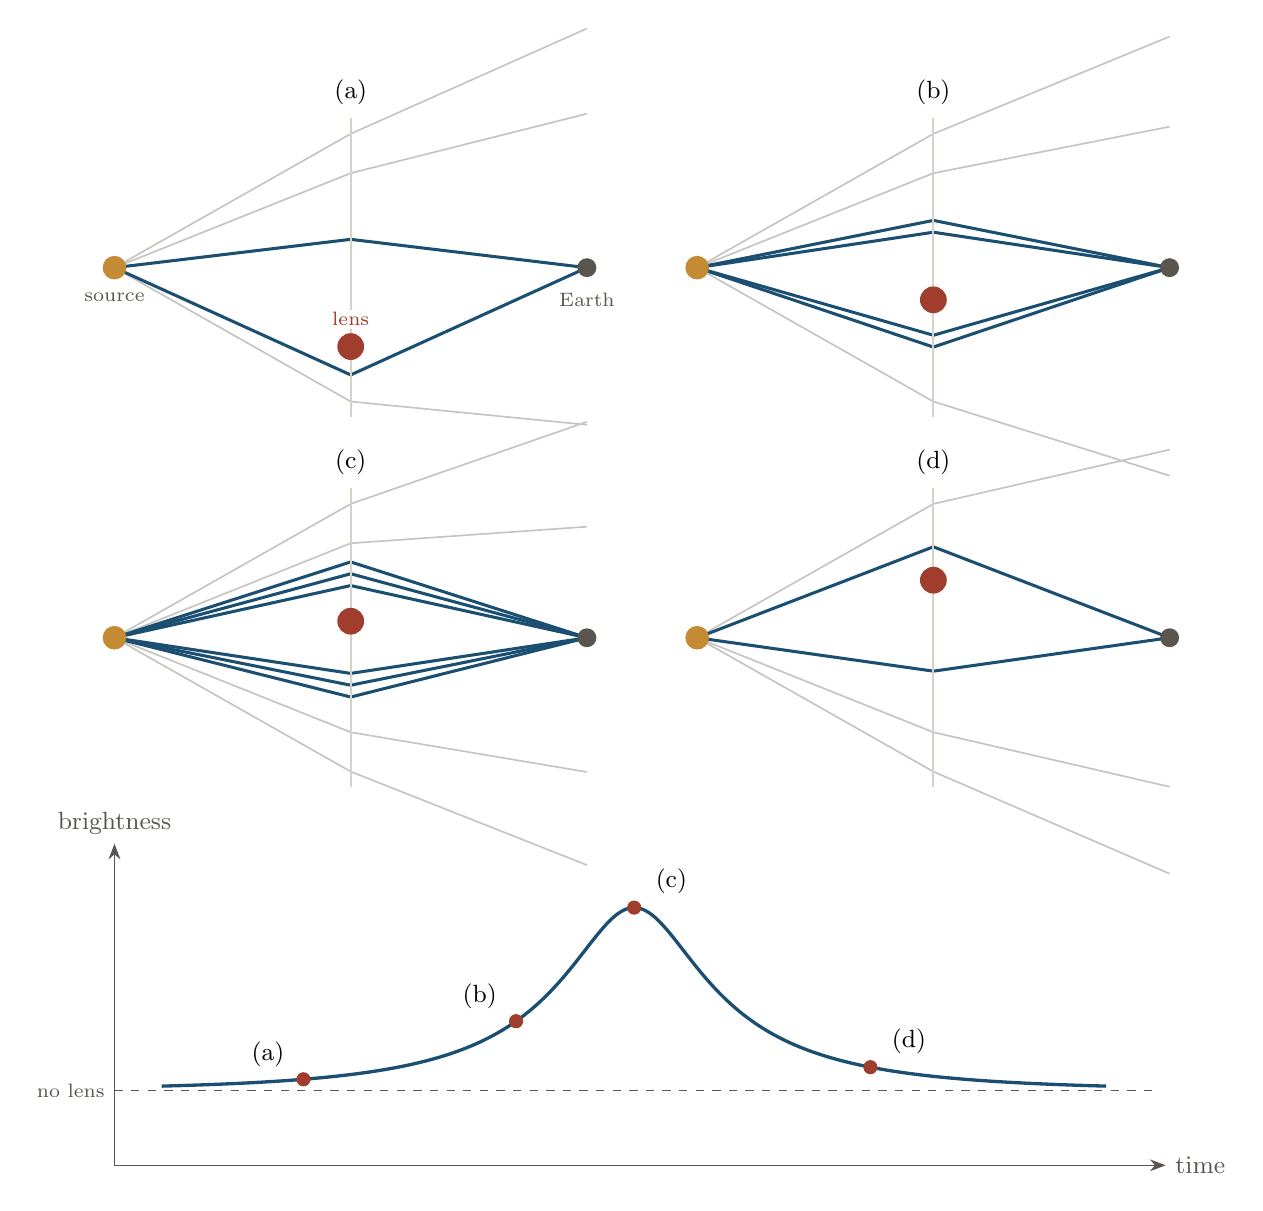
\begin{tikzpicture}[>={Stealth[length=2mm]}]
  \pgfmathsetmacro{\RE}{0.7}
  \pgfmathsetmacro{\dd}{3}
  \pgfmathsetmacro{\kk}{2*\RE*\RE/\dd}
  \pgfmathsetmacro{\uo}{0.3}
  \foreach \t/\lab/\sx/\sy in {-1.4/a/0/0, -0.5/b/7.4/0, 0/c/0/-4.7, 1.0/d/7.4/-4.7}{
    \begin{scope}[shift={(\sx,\sy)}, x=1.0cm, y=1.0cm]
      \pgfmathsetmacro{\u}{sqrt(\uo*\uo+\t*\t)}
      \pgfmathsetmacro{\h}{(\t<0 ? -\u : \u)*\RE}
      \pgfmathsetmacro{\AA}{(\u*\u+2)/(\u*sqrt(\u*\u+4))}
      \pgfmathsetmacro{\sq}{sqrt(\h*\h+4*\RE*\RE)}
      \pgfmathsetmacro{\yp}{(\h+\sq)/2}
      \pgfmathsetmacro{\ym}{(\h-\sq)/2}
      \pgfmathtruncatemacro{\nn}{round(\AA)}
      % grey rays that miss Earth, bent once at the lens plane
      \foreach \y in {-1.7,-1.2,1.2,1.7}{
        \pgfmathparse{(abs(\y-\h)>0.3 && abs(\y-\yp)>0.3 && abs(\y-\ym)>0.3) ? 1 : 0}
        \ifnum\pgfmathresult=1
          \pgfmathsetmacro{\z}{2*\y-\dd*\kk/(\y-\h)}
          \draw[muted!35, line width=0.6pt] (0,0) -- (\dd,\y) -- (2*\dd,\z);
        \fi
      }
      % dark rays bent into Earth, \nn per image
      \foreach \j in {1,...,\nn}{
        \pgfmathsetmacro{\o}{(\j-(\nn+1)/2)*0.15}
        \draw[astroblue, line width=1.1pt] (0,0) -- (\dd,\yp+\o) -- (2*\dd,0);
        \draw[astroblue, line width=1.1pt] (0,0) -- (\dd,\ym+\o) -- (2*\dd,0);
      }
      \draw[linecol, line width=0.8pt] (\dd,-1.9) -- (\dd,1.9);
      \node[circle, fill=sunyellow!85!black, minimum size=3mm, inner sep=0pt] at (0,0) {};
      \node[circle, fill=muted, minimum size=2.4mm, inner sep=0pt] at (2*\dd,0) {};
      \node[circle, fill=accent, minimum size=3.4mm, inner sep=0pt] at (\dd,\h) {};
      \node[font=\small, anchor=south] at (\dd,1.95) {(\lab)};
      \ifnum\pdfstrcmp{\lab}{a}=0
        \node[below, font=\scriptsize, muted] at (0,-0.2) {source};
        \node[below, font=\scriptsize, muted] at (2*\dd,-0.2) {Earth};
        \node[font=\scriptsize, accent, anchor=south, fill=white, inner sep=1pt] at (\dd,\h+0.22) {lens};
      \fi
    \end{scope}
  }
  % ---- light curve
  \begin{scope}[shift={(6.6,-11.4)}, x=3cm, y=0.95cm]
    \draw[->, muted] (-2.2,0) -- (2.25,0) node[right] {\small time};
    \draw[->, muted] (-2.2,0) -- (-2.2,4.3) node[above] {\small brightness};
    \draw[muted, dashed, line width=0.4pt] (-2.2,1) -- (2.2,1);
    \node[left, muted] at (-2.2,1) {\scriptsize no lens};
    \draw[astroblue, line width=1.2pt, domain=-2:2, samples=401]
      plot (\x, {(0.09+\x*\x+2)/(sqrt(0.09+\x*\x)*sqrt(0.09+\x*\x+4))});
    \foreach \t/\lab in {-1.4/a, -0.5/b, 0/c, 1.0/d}{
      \pgfmathsetmacro{\uu}{sqrt(0.09+\t*\t)}
      \pgfmathsetmacro{\AA}{(\uu*\uu+2)/(\uu*sqrt(\uu*\uu+4))}
      \node[circle, fill=accent, minimum size=1.8mm, inner sep=0pt] at (\t,\AA) {};
      \ifdim\t pt<0pt \node[font=\small, anchor=south east] at (\t-0.04,\AA+0.04) {(\lab)};\else\node[font=\small, anchor=south west] at (\t+0.05,\AA+0.05) {(\lab)};\fi
    }
  \end{scope}
\end{tikzpicture}
\end{document}
